%%Chapter - Split into separate file if too large
\chapter{Side Dishes and Extras}

%%Start recipe
\newrecipe{Spiced Sweet Potato Mash}{}

%% \begin{figure}[h!]
%% \centering
%% \includegraphics[scale=0.75]{./img/image.jpg}
%% \end{figure}

\section*{Ingredients}
\begin{ingredients-list}
	\item 2 Sweet Potatoes, approximately same size and thickness
	\item 1 tsp. Cumin seeds
	\item 1 tsp. Caraway seeds
	\item Juice of 1 lemon
\end{ingredients-list}

\section*{Directions}
\begin{enumerate}
	\item Preheat oven to 180 C and line an oven tray with baking paper.
	\item Rub oil liberally over the skin of the sweet potatoes and bake in the oven for 40-60 minutes
		depending on thickness of the sweet potatoes.
	 Remove from the oven and allow to cool for 15-20 minutes.
	\item Dry roast the seeds in a small frypan and grind finely in a mortar and pestle
	\item Make a shallow cut lengthways and peel the skin from the sweet potato.
	\item Place the sweet potato in a bowl and mash coarsely with a fork
	\item  Add the ground spices and mix. Add lemon juice to taste.
\end{enumerate}
Can be served immediately at room temperature, or refrigerated and reheated later.


%%End recipe

%%Start Recipe
\newrecipe{Coconut Rice}{http://www.food.com/recipe/coconut-rice-126690}

\section*{Ingredients}
\begin{ingredients-list}
	\item 1 cup basmati rice
	\item 1 tablespoon olive oil
	\item \sfrac{1}{8} teaspoon salt
	\item 1 pinch saffron (about 5-6 threads)
	\item 1 cup chicken broth
	\item \sfrac{3}{4} cup coconut milk
\end{ingredients-list}

\section*{Directions}
\begin{enumerate}
	\item In a pot that has a tight-fitting lid, over high heat, add the rice, olive oil, salt, and saffron.
		Stirring with a wooden spoon, heat for 2-3 minutes until a few rice grains begin to brown on the edges.
		OPTIONAL: You may want to add a few ounces of shredded coconut at this stage.
	\item Being careful to avoid flare-ups and spill-overs, add the chicken broth and coconut milk to the hot pan. It will sizzle and bubble vigorously!
	\item  Stir to loosen any rice on the bottom or sides of the pot and reduce the heat to low. Put on the lid and cook for 13 minutes.
	\item  When 13 minutes are up, turn off the heat and let the covered rice sit for 5 minutes.
	\item Remove the lid and fluff with a fork before serving with any Asian, Polynesian, or Indian dish.
\end{enumerate}
%%End recipe

%%Start Recipe
\newrecipe{Espinacas con Garbanzos (Spinach \& Chickpeas)}{http://smittenkitchen.com/blog/2010/03/spinach-and-chickpeas/}

\section*{Ingredients}
\begin{ingredients-list}
	\item 2 420g cans of chickpeas, drained and rinsed
	\item 6 tablespoon olive oil
	\item 450g spinach, washed
	\item A hefty 1-inch slice from a country loaf or about 2 slices from sandwich loaf bread (2.5 ounces or 75 grams), crusts removed and cut inset small cubes
	\item \sfrac{1}{2} cup (4 ounces) tomato sauce
	\item 3 garlic cloves, thinly sliced
	\item 1/2 teaspoon ground cumin
	\item Pinch of red pepper flakes
	\item 1 \sfrac{1}{2} tablespoons red wine vinegar
	\item \sfrac{1}{2} teaspoon smoked paprika**
	\item Salt and freshly ground black pepper
	\item Lemon juice, to taste
\end{ingredients-list}

\section*{Directions}
\begin{enumerate}
	\item Place a large saucepan over medium heat and add half the olive oil. When it is hot, add the spinach with a pinch of salt (in batches, if necessary) and stir well.
		Remove when the leaves are just tender, drain in a colander and set aside.
	\item Heat 2 more tablespoons olive oil in a frying pan over medium heat. Fry the bread for about 5 minutes or until golden brown all over,
		 then the remaining tablespoon of oil and the garlic, cumin and pepper. Cook for 1 minute more or until the garlic is nutty brown.
	\item Transfer to a food processor, blender or mortar and pestle along with the vinegar, and mash to a paste. 
		Return the mixture to the pan and add the drained chickpeas and tomato sauce. 
		Stir until the chickpeas have absorbed the flavors and are hot. Season with salt and pepper.
\end{enumerate}
If the consistency is a little thick, add some water. Add the spinach and cook until it is hot. Check for seasoning and serve with paprika on top, or on fried bread toasts (as the Spanish do).
%%End recipe

%%Start recipe
\newrecipe{Spicy Potatoes with Pappadums}{http://www.taste.com.au/recipes/6471/spicy+potatoes+with+pappadums}

%\begin{figure}[h!]
%	\centering
%	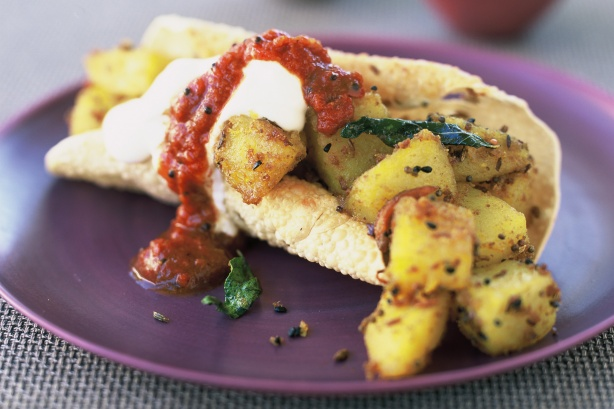
\includegraphics[scale=0.3]{./img/spicypotatoes.jpg}
%\end{figure}

\bigskip
\section*{Ingredients}
\begin{ingredients-list}
	\item 750g potatoes, peeled, cubed
		\begin{textblock*}{8cm}(6.7cm,-1.2cm) % {block width} (coords)
			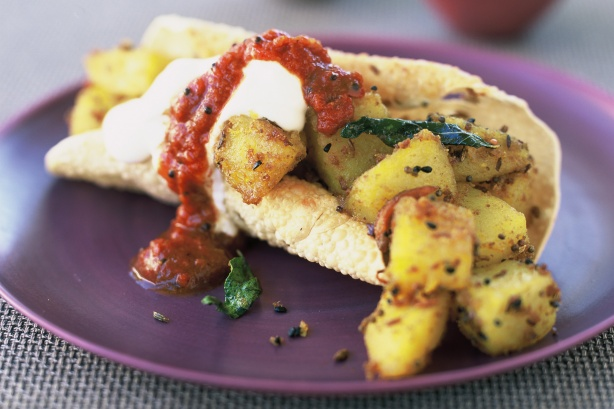
\includegraphics[scale=0.42]{./img/spicypotatoes.jpg}
		\end{textblock*}
	\item 3 tbs ghee (see Notes)
	\item \sfrac{1}{2} tsp turmeric
	\item 2 tbs panch phora 
	\item 1 tbs ground cumin
	\item 6 fresh curry leaves
	\item 1 garlic clove, crushed
	\item 1 tbs grated fresh ginger
	\item 6 large pappadums
	\item 60ml (\sfrac{1}{4} cup) lemon juice
	\item \sfrac{1}{4} cup chopped fresh coriander
	\item Tomato kasundi (see \hyperlink{tomato_kasundi}{related recipe} on page \pageref{tomato_kasundi} ) and yoghurt, if desired, to serve
\end{ingredients-list}

\section*{Directions}
\begin{enumerate}
	\item Place the potatoes in a saucepan of salted water and bring to the boil (alternatively steam them). Cook until just tender. Drain and set aside.
	\item Heat a tablespoon of the ghee in a medium frying pan.
		Add the dry spices, curry leaves, garlic and ginger and cook over medium heat for 1 minute, stirring until the flavours are released.
		Transfer to a bowl and set aside. Add 1 tablespoon of ghee to the pan; when it has melted, add potatoes (in 2 batches if necessary) and cook until golden.
		Return spice mixture to pan and cook for a further minute. Cover and set aside.
	\item Heat remaining ghee in a small frying pan over high heat.
		Carefully place 1 pappadum in the hot oil (press with tongs to help hold the shape) and fry for 2-3 seconds each side until fully expanded.
		Use tongs to transfer to paper towel to drain. Repeat with remaining pappadums.
	\item Add the lemon juice and coriander to the potatoes and reheat gently over low heat for 1-2 minutes.
	\item Place a pappadum on a serving plate, top with some spicy potatoes and the tomato kasundi. Add a dollop of yoghurt.
\end{enumerate}
%%End Recipe

%%Start recipe
\newrecipe{Super Easy Flatbreads}{http://www.jamieoliver.com/recipes/bread-recipes/easy-flatbreads}

\bigskip
\section*{Ingredients}
\begin{ingredients-list}
	\item 350g self-raising flour, plus extra for dusting
		\begin{textblock*}{8cm}(9.7cm,-2.2cm) % {block width} (coords)
			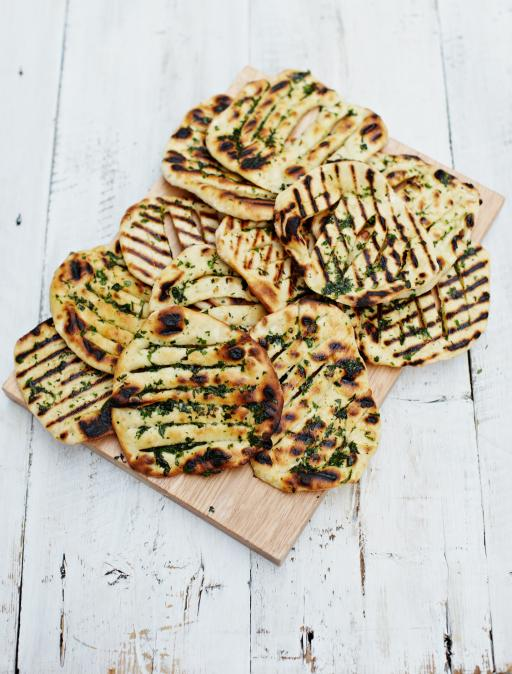
\includegraphics[scale=0.24]{./img/flatbread.jpg}
		\end{textblock*}
	\item sea salt
	\item 1 tsp baking powder
	\item 350g natural yoghurt
\end{ingredients-list}

\section*{Directions}
\begin{enumerate}
	\item Add all the flatbread ingredients to a mixing bowl and mix together with a spoon, then use clean hands to pat and bring everything together.
	\item Dust a clean work surface with flour, then tip out the dough.
	\item Knead for a minute or so to bring it all together (this isn't a traditional bread recipe, so you don't need to knead it for long – just enough time to bring everything together). 
	\item Dust a clean work surface and rolling pin with flour, then divide the dough in half, then divide each half into 6 equal-sized pieces (roughly the size of a golf ball).
	\item With your hands, pat and flatten the dough, then use a rolling pin to roll each piece into 12cm rounds, roughly 2mm to 3mm thick.
	\item Use a knife to cut 6 lines into the centre of each round, leaving about 3cm at each end.
	\item Place the griddle pan on a high heat, then once hot, cook each one for 1 to 2 minutes on each side, or until bar-marked and puffed up, turning with tongs.
	\item Brush the flatbreads all over with herby garlic butter as they come off the griddle, then pile onto a serving board so everyone can dig in and help themselves.
\end{enumerate}
Note that these work just as well without the baking powder or the cutlines in the centre.
%%End Recipe


%%End Chapter